%%%%%%%%%%%%%%%%%%%%%%% file template.tex %%%%%%%%%%%%%%%%%%%%%%%%%
%
% This is a  template file for the LaTeX package SVJour3 width change file svepjc3.clo
% for Springer journal:
% The European Physical Journal C
%
% Copy it to a new file with a new name and use it as the basis
% for your article. Delete % signs as needed.
%
% This template includes a few options for different layouts and
% content for various journals. Please consult a previous issue of
% your journal as needed.
%
%%%%%%%%%%%%%%%%%%%%%%%%%%%%%%%%%%%%%%%%%%%%%%%%%%%%%%%%%%%%%%%%%%%
%
\RequirePackage{rotating}
\RequirePackage{fix-cm}
%
\documentclass[twocolumn,epjc3]{svjour3}  
%
\smartqed  % flush right qed marks, e.g. at end of proof
%
\RequirePackage{graphicx}
%
% \RequirePackage{mathptmx}      % use Times fonts if available on your TeX system
%
% insert here the call for the packages your document requires
%\RequirePackage{latexsym}
%\RequirePackage[sort&compress,numbers]{natbib}
%\RequirePackage[colorlinks,citecolor=blue,urlcolor=blue,linkcolor=blue]{hyperref}
%\RequirePackage{lineno}
\RequirePackage[switch,modulo]{lineno}
\RequirePackage{hyperref}
\RequirePackage{amsmath}
\RequirePackage{hepnames}
\RequirePackage{bm}
\RequirePackage{multirow}
\RequirePackage{amssymb}
\RequirePackage{xspace}
\RequirePackage{rotating}
% etc.
%
% please place your own definitions here and don't use \def but
% \newcommand{}{}
\newcommand{\PZggx}{\ensuremath{\PZ/\Pgamma^{*}}\xspace}
\newcommand{\pT}{\ensuremath{p_{\textrm{T}}}\xspace}
\newcommand{\pThat}{\ensuremath{\hat{p}_{\textrm{T}}}\xspace}
\newcommand{\kt}{\ensuremath{k_{\textrm{t}}}\xspace}
\newcommand{\HT}{\ensuremath{H_{\mathrm{T}}}\xspace}
\newcommand{\GeV}{\ensuremath{\textrm{GeV}}\xspace}
\newcommand{\TeV}{\ensuremath{\textrm{TeV}}\xspace}
\newcommand{\data}{\ensuremath{\textrm{data}}\xspace}
\newcommand{\mc}{\ensuremath{\textrm{mc}}\xspace}
\newcommand{\incl}{\ensuremath{\textrm{incl}}\xspace}
\newcommand{\jet}{\ensuremath{\textrm{jet}}\xspace}
\newcommand{\pileup}{\ensuremath{\textrm{PU}}\xspace}
\newcommand{\Poisson}{\ensuremath{\textrm{Poisson}}\xspace}
\newcommand{\Nbar}{\ensuremath{\bar{N}}\xspace}
\newcommand{\Born}{\ensuremath{\textrm{born}}\xspace}
\newcommand{\ME}{\ensuremath{\textrm{me}}\xspace}
\newcommand{\MGvATNLO}{\textsc{MadGraph5}\_aMC@NLO\xspace}
\newcommand{\PYTHIA}{\textsc{Pythia}\xspace}
\newcommand{\POWHEG}{\textsc{Powheg}\xspace}
\newcommand{\ALPGEN}{\textsc{Alpgen}\xspace}
\newcommand{\SHERPA}{\textsc{Sherpa}\xspace}
\newcommand{\FEWZ}{\textsc{FEWZ}\xspace}
\newcommand{\MCFM}{\textsc{MCFM}\xspace}
\newcommand{\cf}{cf.\xspace}
\newcommand{\ie}{i.e.\xspace}
\newcommand{\eg}{e.g.\xspace}
\newcommand{\fbinv}{\ensuremath{\textrm{~fb}^{-1}}\xspace}
%
\journalname{Eur. Phys. J. C}
%
\begin{document}

\title{Stitching Monte Carlo samples%\thanksref{t1}
}
%\subtitle{Do you have a subtitle?\\ If so, write it here}

%\titlerunning{Short form of title}        % if too long for running head

\author{Karl Ehat\"aht\thanksref{e1,addr1}
        \and
        Christian Veelken\thanksref{e2,addr1} %etc.
}


%\thankstext{t1}{Grants or other notes
%about the article that should go on the front page should be
%placed here. General acknowledgments should be placed at the end of the article.
\thankstext{e1}{e-mail: karl.ehataht@cern.ch}
\thankstext{e2}{e-mail: christian.veelken@cern.ch}

%\authorrunning{Short form of author list} % if too long for running head

\institute{National Institute of Chemical Physics and Biophysics (NICPB), Akadeemia tee 23, 12618 Tallinn, Estonia \label{addr1}
}

\date{Received: date / Accepted: date}
% The correct dates will be entered by the editor

\maketitle

\linenumbers

\begin{abstract}
%Insert your abstract here. Include keywords, PACS and mathematical
%subject classification numbers as needed.
Monte Carlo (MC) simulations are extensively used for various purposes in modern high-energy physics (HEP) experiments.
Precise measurements of established Standard Model processes or searches for new physics often require the collection of vast amounts of data.
It is often difficult to produce MC samples of size matching that of the data, as substantial computing resources are required to produce and store such samples.
One solution often employed when producing MC samples for HEP experiments 
is to divide the phase-space of particle interactions into multiple regions 
and produce the MC samples separately for each region,
with the size of MC samples being adapted to the needs of physics analyses that are performed in these regions.
In this paper we present an optimal procedure for combining MC samples that overlap in phase-space.
Our procedure is optimal in the sense that it provides the lowest statistical uncertainties.
We refer to the procedure as ``stitching''.
The paper includes different examples for applying the procedure to simulated proton-proton collisions at the CERN Large Hadron Collider.
%\keywords{First keyword \and Second keyword \and More}
% \PACS{PACS code1 \and PACS code2 \and more}
% \subclass{MSC code1 \and MSC code2 \and more}
\end{abstract}

\section{Introduction}
\label{sec:introduction}

Monte Carlo (MC) simulations~\cite{Kroese2014WhyTM,dunn2011exploring} are used for a plethora of different purposes in contemporary high-energy physics (HEP) experiments.
Applications for experiments currently in operation include detector calibration; optimization of analysis techniques, including the training of machine learning algorithms;
the modelling of backgrounds, as well as the modelling of signal acceptance and efficiency.
Besides, MC simulations are extensively used for detector development and for estimating the physics reach of experiments that are presently in construction or planned in the future.
When using MC simulations for the purpose of modelling background contributions,
the production of sufficiently large MC samples often poses a material challenge in terms of the computing resources required to produce and store such samples.

This is especially true for experiments at the CERN Large Hadron Collider (LHC)~\cite{Bruning:2004ej,Buning:2004wk,Benedikt:2004wm},
firstly due to the large cross section of proton-proton ($\Pp\Pp$) collisions and secondly due to the large luminosity delivered by the LHC.
We refer to a single $\Pp\Pp$ collision as an ``event''.
The number of events, $N_{\data}$, produced within a given interval of time 
is given by the product of the $\Pp\Pp$ scattering cross section, $\sigma$, and of the integrated luminosity, $L$, that the LHC has delivered during this time:
$N_{\data} = \sigma \times L$.
The inelastic $\Pp\Pp$ scattering cross section at the present LHC center-of-mass energy of $\sqrt{s}=13$~\TeV amounts to $\approx 75$~mb~\cite{Aaboud:2016mmw,Sirunyan:2018nqx},
while the integrated luminosities recorded at $\sqrt{s}=13$~\TeV by the ATLAS and CMS experiments amount to $\approx 140\fbinv$~\cite{ATLAS-CONF-2019-021,LUM-17-001,LUM-17-004,LUM-18-002}.
Thus, $N_{\data} \approx 10^{16}$ inelastic $\Pp\Pp$ scattering events occurred in each of the two experiments during this time.

In order to render the statistical uncertainties on background estimates obtained from the MC simulation small compared to the statistical uncertainties on the data,
MC samples of size larger than $N_{\data}$ are needed, ideally $N_{\mc} \gtrsim 10 \times N_{\data}$,
where the size of the MC sample is denoted by the symbol $N_{\mc}$.
Such large MC samples are prohibitive to produce.
The solution to this apparent dilemma is to restrict the production of MC samples to the processes most relevant for physics analyses,
which typically focus on events that contain either charged leptons, jets of high transverse momentum ($\pT$), or high $\pT$ neutrinos,
where the latter is indicated by the presence of large missing transverse momentum in the event.
The cross sections of these processes are orders of magnitude lower compared to the inelastic $\Pp\Pp$ scattering cross section~\footnote{ 
See Ref.~\cite{StandardModelCrossSections} for a summary of Standard Model cross sections relevant for physics analyses at the LHC.}.
Elaborate MC production schemes are in common use at the LHC.
These schemes typically restrict the set of MC samples to those processes most relevant for physics analyses.

The production of MC samples of sufficient size is of particular importance in searches for new physics.
In these searches, potential signals are typically expected to be small
compared to the background contributions arising from established Standard Model (SM) processes
and the presence or absence of a signal may in fact be obscured by the statistical uncertainties on the background estimate,
unless MC samples of adequate size are available to model the main background processes~\footnote{
The presence of large signals is often already excluded by the results of previous searches, based on a smaller dataset.}.
Searches for new physics are often performed in phase-space (PS) regions that are atypical for background processes,
as only in these regions the ratio $S/\sqrt{B}$ is sufficiently large to allow for the discovery of potential signals.
The MC production schemes employed by the ATLAS and CMS experiments take advantage of the fact 
that often only a small percentage of the background populates the regions of PS most relevant for physics analyses.
A typical strategy is to divide the PS into multiple regions and to produce separate MC samples for each region.
The size of MC samples covering each region is then chosen such to be as small as possible,
while keeping the statistical uncertainties on the background estimates obtained from these samples at an acceptable level.
The choice of the regions is driven by the needs of physics analyses.

The sets of MC samples produced following this strategy often overlap in PS,
as a consequence of different schemes being used for dividing the PS into distinct regions by different physics analyses.
For example, one set of MC samples may divide the PS based on the number of jets, 
whereas another set of MC samples may divide the PS based on $\HT$, the scalar sum in $\pT$ of the jets in the event.
In this paper, we present a procedure for combining MC samples in an ``optimal'' way,
where optimal refers to yielding the lowest statistical uncertainty on the background estimate that can be achieved when combining a given set of MC samples.
Our formalism handles the case that different MC samples may use different schemes to divide the PS into distinct regions,
thereby allowing to use all available MC samples, regardless of any arbitrary overlap in PS between these samples.
The overlap between MC samples in PS is accounted for by applying appropriately chosen weights to simulated events.
We refer to this procedure as ``stitching''.

The structure of this paper is as follows:
the formalism for computing the stitching weights is developed in Section~\ref{sec:stitching_weights}.
In Section~\ref{sec:examples}, we present examples for applying the formalism to $\Pp\Pp$ collisions at the LHC.
The paper concludes with a summary in Section~\ref{sec:summary}.


\section{Computation of stitching weights}
\label{sec:stitching_weights}

As explained in the introduction,
contemporary HEP experiments often employ MC production schemes
that first divide the PS into multiple regions and then produce separate MC samples to cover each region.
When using these MC samples for the purpose of modelling backgrounds,
weights need to be applied to the simulated events, in order to obtain background estimates that are unbiased.
More specifically, the weights need to be chosen such that the weighted sum of simulated events in each region $i$ of PS 
matches the SM prediction in that region:
\begin{equation}
\sum_{j} \, N_{j} \times P_{j}^{i} \times w_{j}^{i} = L \times \sigma_{i} \, ,
\label{eq:one}
\end{equation}
where the symbol $L$ corresponds to the integrated luminosity of the analyzed dataset
and $\sigma_{i}$ denotes the fiducial cross section for the process under study in the PS region $i$.
The sum on the left-hand-side extends over the MC samples $j$,
with $N_{j}$ denoting the total number of simulated events in the $j$-th sample.
The symbol $P_{j}^{i}$ corresponds to the probability for an event in MC sample $j$ to fall into PS region $i$,
and $w_{j}^{i}$ denotes the weight that is applied to events from the $j$-th sample,
which falls into the PS region $i$.
Eq.~(\ref{eq:one}) holds separately for each background process under study.
In principle, the same equation applies to signal MC samples. 
The case of signal MC samples is less relevant in practice, however,
as signal cross sections are typically significantly smaller than those of background processes,
and the production of signal MC samples of sufficient size is rarely a problem.

One can show that the lowest statistical uncertainty on the background estimate is achieved 
if the weights $w_{j}^{i}$ in Eq.~(\ref{eq:one}) only depend on the PS region $i$,
that is, if all simulated events that fall into the same region of PS have the same weight,
regardless of which MC sample these events are contained in.
We hence use weights that depend only on the PS region $i$ and not on the MC sample $j$.
We refer to these weights as ``stitching weights'' and denote them by the symbol $w^{i}$.

It is useful to express the cross section $\sigma_{i}$ as the product of an ``inclusive'' cross section $\sigma_{\incl}$,
which refers to the whole PS, and the probability $P^{i}$ that an event generated in the inclusive PS falls into the PS region $i$:
\begin{equation*}
\sigma_{i} = \sigma_{\incl} \times P^{i} \, .
\label{eq:two}
\end{equation*}
Inserting this relation into Eq.~(\ref{eq:one}) and solving for the weight $w^{i}$ yields:
\begin{equation}
w^{i} = \frac{L \times \sigma_{\incl} \times P^{i}}{\sum_{j} \, N_{j} \times P_{j}^{i}} \, .
\label{eq:master}
\end{equation}

A special case, which is frequently encountered in practice,
is that one MC sample covers the whole PS,
while additional samples reduce the statistical uncertainties in the regions of PS most relevant to searches for new physics.
We refer to the MC sample that covers the whole PS as the inclusive sample and the corresponding PS as the inclusive PS.
In this case, Eq.~(\ref{eq:master}) can be rewritten in the form:
\begin{equation}
w^{i} = \frac{L \times \sigma_{\incl}}{N_{\incl}} \times \frac{N_{\incl} \times P^{i}}{N_{\incl} \times P^{i} + \sum_{j} \, N_{j} \times P_{j}^{i}} \, ,
\label{eq:weight_incl}
\end{equation}
where $N_{\incl}$ refers to the number of events in the inclusive sample.
The sum over $j$ in Eq.~(\ref{eq:weight_incl}) extends over the additional samples that each cover a different region in PS
and to which we will refer to as ``exclusive'' samples.
The two factors in Eq.~(\ref{eq:weight_incl}) may be interpreted in the following way:
the first factor corresponds to the weights that one would apply to the events in PS region $i$ 
in case no exclusive samples are available and the background estimate in PS region $i$ is based solely on the inclusive sample.
The availability of the additional exclusive samples increases the number of simulated events in the PS region $i$ 
from $N_{\incl} \times P^{i}$ to $N_{\incl} \times P^{i} + \sum_{j} \, N_{j} \times P_{j}^{i}$,
thereby reducing the weights applied to simulated events that fall into this region.
The resulting reduction in weights is given by the second factor in Eq.~(\ref{eq:weight_incl}).

We note in passing that the square-root of this factor,
$\sqrt{\frac{N_{\incl} \times P^{i}}{N_{\incl} \times P^{i} + \sum_{j} \, N_{j} \times P_{j}^{i}}}$,
constitutes the quantity most relevant for physics analyses,
as it represents the reduction in statistical uncertainty on the background estimate in PS region $i$
that results from the availability of the additional exclusive samples and the application of our stitching procedure.


\section{Examples}
\label{sec:examples}

In this Section, we illustrate the formalism developed in Section~\ref{sec:stitching_weights} with concrete examples,
drawn from two different applications: the estimation of 
%Drell-Yan (DY) and 
$\PW$+jets backgrounds in physics analyses at the LHC
and the estimation of trigger rates for the high-luminosity LHC (HL-LHC) upgrade~\cite{TDR_Phase2_LHC},
scheduled to start operation in 2027.

The 
%DY production of lepton pairs ($\PZggx \to \Plepton\Plepton$) as well as the 
production of $\PW$ bosons with subsequent decay to a charged lepton and a neutrino ($\PW \to \Plepton\Pnu$)
%constitute 
constitutes a relevant backgrounds to many physics analyses at the LHC,
for example the analysis of SM Higgs ($\PHiggs$) boson production in the decay 
%modes $\PHiggs \to \Pgt\Pgt$ and 
mode $\PHiggs \to \PW\PW$
and the search for $\PHiggs$ boson pair production in the decay 
%modes $\PHiggs\PHiggs \to \Pbottom\Pbottom\Pgt\Pgt$ and 
%$\PHiggs\PHiggs \to \Pbottom\Pbottom\PW\PW$~\cite{ATLAS:2014aga,Aad:2015vsa,Aad:2019yxi,Aaboud:2018sfw,CMS-HIG-13-004,CMS-HIG-13-027,CMS-HIG-17-002,CMS-HIG-17-006}.
mode $\PHiggs\PHiggs \to \Pbottom\Pbottom\PW\PW$~\cite{ATLAS:2014aga,Aad:2019yxi,CMS-HIG-13-027,CMS-HIG-17-006}.
Simulated samples of $\PW$+jets 
%and DY 
events have been produced for $\Pp\Pp$ collisions at $\sqrt{s}=13$~\TeV center-of-mass energy
using matrix elements computed at leading order (LO) 
%and at next-to-leading order (NLO) 
accuracy in perturbative quantum chromodynamics (pQCD)
with the program \MGvATNLO $2.6.5$~\cite{MGvATNLO}.
The parton distribution functions of the proton are modeled with NNPDF3.1 set~\cite{NNPDF:2017mvq}.
%The production of DY events is restricted to the fiducial region $m_{\Plepton\Plepton} > 50$~\GeV, where $m_{\Plepton\Plepton}$ denotes the mass of the lepton pair.
Parton showering, hadronization, and the underlying event are modeled using the program \PYTHIA $v8.2$~\cite{PYTHIA} with the tune \textrm{CP5}~\cite{Sirunyan:2019dfx}.
The matching of matrix elements to parton showers is done using the \textrm{MLM} scheme~\cite{Alwall:2007fs}.% for the LO samples
%and the \textrm{FXFX} scheme~\cite{Frederix:2012ps} for the NLO samples.
The 
%DY and $\PW$+jets 
samples are normalized using cross sections computed at next-to-next-to leading order (NNLO) accuracy in pQCD,
with electroweak corrections taken into account up to NLO accuracy~\cite{Li:2012wna}.
%The product of the DY cross section in the PS region $m_{\Plepton\Plepton} > 50$~\GeV
%times the branching fraction for the decay into two charged leptons amounts to $6.08$~nb,
%while the cross section for $\PW$+jets production times the branching fraction for the decay to charged lepton and neutrino amounts to $61.5$~nb.
The product of the $\PW$+jets production cross section times the branching fraction for the decay to a charged lepton and a neutrino amounts to $61.5$~nb.

We will demonstrate the stitching of these samples based on two observables,
$N_{\jet}$ and $\HT$, defined as, respectively, the number of jets and the scalar sum in $\pT$ of jets in the event.
The PS region in which we perform the stitching will be either one- or two-dimensional.
We will show that for our formalism
it makes little difference whether the stitching is performed in one dimension or in two:
The regions in PS are enumerated by a single index $i$ in either case,
and in either case the probability $P^{i}$ follows a categorical distribution.

The task of estimating trigger rates for the upcoming high-luminosity data-taking period of the LHC is chosen as second example to illustrate the stitching procedure.
The ``rate'' of a trigger corresponds to the number of $\Pp\Pp$ collision events that satisfy the trigger condition per unit of time.
The estimation of trigger rates constitutes an important task for demonstrating the physics potential of the HL-LHC.
The HL-LHC physics program demands a large amount of integrated luminosity to be delivered by the LHC, 
in order to facilitate measurements of rare signal processes,
such as the precise measurement of $\PHiggs$ boson couplings and the study of $\PHiggs$ boson pair production, by the ATLAS and CMS experiments.
In order to satisfy this demand, the HL-LHC is expected to operate at an instantaneous luminosity of $5$-$7.5 \times 10^{34}$~cm$^{-2}$~s$^{-1}$
at a center-of-mass energy of $\sqrt{s} = 14$~\TeV~\cite{TDR_Phase2_LHC}.
The challenge of developing triggers for the HL-LHC is to design the triggers such that rare signal processes pass the triggers with a high efficiency,
while the rate of background processes gets reduced by many orders of magnitude, in order not to exceed bandwidth limitations on the detector read-out 
and on the rate with which events can be written to permanent storage.

The inelastic $\Pp\Pp$ scattering cross section at $\sqrt{s} = 14$~\TeV amounts to $\approx 80$~mb,
resulting in up to $200$ simultaneous $\Pp\Pp$ interactions per crossing of the proton beams at the nominal HL-LHC instantaneous luminosity~\cite{TDR_Phase2_LHC}.
The vast majority of these interactions are inelastic $\Pp\Pp$ scatterings with low momentum exchange,
which predominantly arise from the exchange of gluons between the colliding protons.
We refer to inelastic $\Pp\Pp$ scattering interactions with no further selection applied as ``minimum bias'' events.
In order to estimate the rates of triggers at the HL-LHC,
MC samples of minimum bias events are produced at LO in pQCD using the program \PYTHIA $v8.2$.
The minimum bias samples are complemented by samples of inelastic $\Pp\Pp$ scattering interactions
in which a significant amount of transverse momentum, denoted by the symbol $\pThat$, is exchanged between the scattered protons.
The stitching of the minimum bias samples with samples generated for different ranges in $\pThat$ allows to estimate the trigger rates with lower statistical uncertainties.

The production of MC samples used for estimating trigger rates at the HL-LHC
proceeds by first simulating one ``hard-scatter'' (HS) interaction within a given range in $\pThat$
and then adding a number of additional inelastic $\Pp\Pp$ scattering interactions of the minimum bias kind to the same event.
We refer to these additional inelastic $\Pp\Pp$ scattering interactions as ``pileup'' (PU)
and use the symbol $N_{\pileup}$ to denote the total number of these additional inelastic $\Pp\Pp$ scattering interactions 
that occur in the same crossing of the proton beams as the HS interaction.
No selection on $\pThat$ is applied when simulating the PU interactions.
The distinction between the HS interaction and the PU interactions is artificial and solely made for the purpose of MC production.
In the data that will be recorded at the HL-LHC, the HS interaction and the PU interactions will be indistinguishable.
The scattering in which the transverse momentum exchange between the protons amounts to $\pThat$ may occur in any of the $N_{\pileup} + 1$ simultaneous $\Pp\Pp$ interactions.
Our formalism treats the HS interaction and the $N_{\pileup}$ additional PU interactions on an equal footing.
We enumerate the regions in PS of the HS and of the PU interactions by a vector $I$ of dimension $N_{\pileup} + 1$.
The $k$-th component of this vector indicates the range in $\pThat$ of the $k$-th $\Pp\Pp$ interaction.
The probability $P^{I} = P^{i_{1},\dots,i_{N_{\pileup}+1}}$ follows a multinomial distribution.


%\subsection{Estimation of DY and \texorpdfstring{$\PW$}{W}+jets backgrounds}
\subsection{Estimation of \texorpdfstring{$\PW$}{W}+jets backgrounds}
\label{sec:examples_background_yield}

The examples in this section refer to the modelling of 
%DY and 
$\PW$+jets backgrounds in the context of physics analyses at the LHC.
We will first discuss the stitching of $\PW \to \Plepton\Pnu$ samples
%generated at LO accuracy in pQCD 
based on the observable $N_{\jet}$
%, followed by a discussion of the stitching of $\PW \to \Plepton\Pnu$ samples generated at LO accuracy in pQCD based on the two observables $N_{\jet}$ and $\HT$,
%before we conclude this section with a discussion of stitching $\PZggx \to \Plepton\Plepton$ samples generated at NLO in pQCD based on the multiplicity of jets.
and then proceed to discuss the stitching of $\PW \to \Plepton\Pnu$ samples based on the two observables $N_{\jet}$ and $\HT$.
In 
%all three 
both cases, we will assume that an inclusive sample, covering the whole PS, is available.


%\subsubsection{Stitching of LO \texorpdfstring{$\PW$}{W}+jets samples by \texorpdfstring{$N_{\jet}$}{Njet}}
\subsubsection{Stitching of \texorpdfstring{$\PW$}{W}+jets samples by \texorpdfstring{$N_{\jet}$}{Njet}}
\label{sec:WJets_vs_Njet}

In this example, an inclusive $\PW \to \Plepton\Pnu$ sample simulated at LO accuracy in pQCD 
is stitched with exclusive samples produced for jet multiplicities of $N_{\jet} = 1$, $2$, $3$, and $4$.
The inclusive sample contains events with jet multiplicities between $0$ and $4$.
We divide the PS by the number of jets and set the index $i$ equal to $N_{\jet}$.
The number of events in each MC sample and the values of the $P^{i}$ and $P_{j}^{i}$ are given in 
%Table~\ref{tab:samples_and_probabilities_WJets_vs_Njet}.
Tables~\ref{tab:samples_WJets_vs_Njet} and~\ref{tab:probabilities_WJets_vs_Njet}.
The number of events in each exclusive sample is chosen to be about an order of magnitude greater
than would be expected from the inclusive sample in the same phase space region.
The probabilities $P^{1}$,$\ldots$,$P^{4}$ are computed by taking the ratio of cross sections 
for the $N_{\jet} = 1$,$\ldots$,$4$ samples with respect to the cross section $\sigma_{\incl}$ of the inclusive sample.
The cross sections used for computing these ratios have been calculated at LO accuracy in pQCD using the program \MGvATNLO
and have been upgraded to NNLO accuracy by scaling all cross sections by the ratio ($k$-factor) of the NNLO to LO inclusive cross sections.
The probability $P^{0}$ is obtained using the relation $P^{0} = 1 - \sum_{i=1}^{4} P^{i}$.
The probabilities $P_{j}^{i}$ for the exclusive samples are $1$ if $i=j$ and $0$ otherwise,
as each of the exclusive samples $j$ covers exactly one of the PS regions $i$.
The corresponding stitching weights, computed according to Eq.~(\ref{eq:weight_incl}), are given in Table~\ref{tab:weights_WJets_vs_Njet}.

Except for the $N_{\jet} = 3$ and $N_{\jet} = 4$ regions,
the weights $w^{i}$ decrease as the number of jets increases, 
reflecting the reduction in statistical uncertainty that is achieved by using the exclusive samples in combination with the inclusive one.
The weights $w^{3}$ and $w^{4}$ for the $N_{\jet} = 3$ and $N_{\jet} = 4$ regions are about the same,
reflecting the fact that the number of events in the $N_{\jet} = 4$ sample is smaller compared to the number of events in the $N_{\jet} = 3$ sample
by about the same factor as the ratio of the corresponding cross sections.

In order to demonstrate that the stitching procedure yields background estimates that are unbiased,
we show distributions in $\pT$ of the ``leading'' and ``subleading'' jet (the jets of, respectively, highest and second-highest $\pT$ in the event),
in the multiplicity of jets and in the observable $\HT$ 
for the inclusive sample and for the sum of inclusive plus exclusive samples in Fig.~\ref{fig:controlPlots_WJets_vs_Njet}.
Jets are reconstructed using the anti-\kt algorithm~\cite{Cacciari:2008gp,Cacciari:2011ma} with a distance parameter of $0.4$,
using all stable particles except neutrinos as input, and are required to satisfy the selection criteria $\pT > 25$~\GeV and $\vert\eta\vert < 5.0$.
The distributions are normalized to an integrated luminosity of $140$~fb$^{-1}$, recorded at $\sqrt{s}=13$~\TeV.
Individual exclusive samples $j$ are distinguished by different colors and fill patterns in the upper part of each figure.
In the lower part, we show the difference between the background prediction obtained from the inclusive sample and from the sum of inclusive and exclusive samples,
using our stitching procedure.
The differences are given relative to the $\PW$+jets background estimate obtained from our stitching procedure.
The size of statistical uncertainties on the background estimates obtained from the inclusive sample and obtained from our stitching procedure
is visualized in the lower part of each figure and is represented by the the length of the error bars and by the height of the dark shaded area, respectively.

The distributions for the inclusive sample and for the sum of inclusive plus exclusive samples, with the stitching weights applied, are in agreement within the statistical uncertainties.
The exclusive samples reduce the statistical uncertainties in particular in the tails of the distributions,
which are the regions most relevant in searches for new physics.

\begin{table}
\caption{
  Number of events in the inclusive $\PW \to \Plepton\Pnu$ sample and in the $\PW \to \Plepton\Pnu$ samples produced in bins of jet multiplicity,
  and corresponding cross sections.
}
\label{tab:samples_WJets_vs_Njet}
\begin{center}
\begin{tabular}{l|c|c|c}
\hline
\multirow{2}{12mm}{Sample} & Index & Number    & Cross                    \\
                           & $j$   & of events & section [nb]$^{\dagger}$ \\
\hline
Inclusive                  & $-$   & $3 \times 10^{6}$ & $61.5$           \\
\hline
$N_{\jet} = 1$             & $1$   & $4.9 \times 10^{6}$ & $10.1$           \\
$N_{\jet} = 2$             & $2$   & $1.6 \times 10^{6}$ & $3.21$           \\
$N_{\jet} = 3$             & $3$   & $4.6 \times 10^{5}$ & $0.938$          \\
$N_{\jet} = 4$             & $4$   & $2.2 \times 10^{5}$ & $0.443$          \\
\hline
\end{tabular}
\end{center}
$^{\dagger}$ Computed at LO accuracy in pQCD, then scaled to NNLO
\end{table}

\begin{table}
\caption{
  Probabilities $P^{i}$ for the events in the inclusive and exclusive samples to populate the different PS regions $i$.
  The PS regions $i$ are defined by the observable $N_{\jet}$, the number of jets.
}
\label{tab:probabilities_WJets_vs_Njet}
\begin{center}
\begin{tabular}{l|ccccc}
\hline
\multirow{2}{12mm}{Sample} & \multicolumn{5}{c}{Probabilities}               \\
                           & $P^{0}$ & $P^{1}$ & $P^{2}$ & $P^{3}$ & $P^{4}$ \\
\hline
Inclusive                  & $0.755$ & $0.169$ & $0.053$ & $0.016$ & $0.007$ \\
\hline
$N_{\jet} = 1$             & $0$     & $1$     & $0$     & $0$     & $0$     \\
$N_{\jet} = 2$             & $0$     & $0$     & $1$     & $0$     & $0$     \\
$N_{\jet} = 3$             & $0$     & $0$     & $0$     & $1$     & $0$     \\
$N_{\jet} = 4$             & $0$     & $0$     & $0$     & $0$     & $1$     \\
\hline
\end{tabular}
\end{center}
\end{table}

\begin{table}
\caption{
  Weights $w^{i}$ for the case that the inclusive and exclusive $\PW \to \Plepton\Pnu$ samples 
  given in Table~\ref{tab:samples_WJets_vs_Njet}
  are stitched based on $N_{\jet}$, the number of jets.
  The weights are computed for an integrated luminosity of $140\fbinv$.
}
\label{tab:weights_WJets_vs_Njet}
\begin{center}
\begin{tabular}{l|ccccc}
\hline
 & \multicolumn{5}{c}{Multiplicity of jets} \\
 & $0$ & $1$ & $2$ & $3$ & $4$ \\
\hline
Weight & $2870$ & $264$ & $255$ & $260$ & $259$ \\
\hline
\end{tabular}
\end{center}
\end{table}

%\begin{table*}
%\caption{
%  Number of events in the inclusive $\PW \to \Plepton\Pnu$ sample and in the $\PW \to \Plepton\Pnu$ samples produced in bins of jet multiplicity,
%  corresponding cross sections,
%  and probabilities $P^{i}$ for the events in the inclusive and exclusive samples to populate the different PS regions $i$.
%}
%\label{tab:samples_and_probabilities_WJets_vs_Njet}
%\begin{center}
%\begin{tabular}{l|c|c|c|ccccc}
%\hline
%\multirow{2}{12mm}{Sample} & Index & Number    & Cross                    & \multicolumn{5}{c}{Probabilities}               \\
%                           & $j$   & of events & section [nb]$^{\dagger}$ & $P^{0}$ & $P^{1}$ & $P^{2}$ & $P^{3}$ & $P^{4}$ \\
%\hline
%Inclusive                  & $-$   & $3 \times 10^{6}$ & $61.5$ & $0.755$ & $0.169$ & $0.053$ & $0.016$ & $0.007$ \\
%\hline
%$N_{\jet} = 1$             & $1$   & $4.9 \times 10^{6}$ & $10.1$  & $0$     & $1$     & $0$     & $0$     & $0$     \\
%$N_{\jet} = 2$             & $2$   & $1.6 \times 10^{6}$ & $3.21$  & $0$     & $0$     & $1$     & $0$     & $0$     \\
%$N_{\jet} = 3$             & $3$   & $4.6 \times 10^{5}$ & $0.938$ & $0$     & $0$     & $0$     & $1$     & $0$     \\
%$N_{\jet} = 4$             & $4$   & $2.2 \times 10^{5}$ & $0.443$ & $0$     & $0$     & $0$     & $0$     & $1$     \\
%\hline
%\end{tabular}
%\end{center}
% $^{\dagger}$ Computed at LO accuracy in pQCD, then scaled to NNLO
%\end{table*}

\begin{figure*}
\setlength{\unitlength}{1mm}
\begin{center}
\begin{picture}(180,182)(0,0)
\put(8.5, 100.0){\mbox{\includegraphics*[height=82mm]{plots/WJets_Njet_lead_stack_wRatio_log.pdf}}}
\put(96.5, 100.0){\mbox{\includegraphics*[height=82mm]{plots/WJets_Njet_sublead_stack_wRatio_log.pdf}}}
\put(8.5, 4.0){\mbox{\includegraphics*[height=82mm]{plots/WJets_Njet_njet_stack_wRatio_log.pdf}}}
\put(96.5, 4.0){\mbox{\includegraphics*[height=82mm]{plots/WJets_Njet_ht_stack_wRatio_log.pdf}}}
\put(45.0, 96.0){\small (a)}
\put(133.0, 96.0){\small (b)}
\put(45.0, 0.0){\small (c)}
\put(133.0, 0.0){\small (d)}
\end{picture}
\end{center}
\caption{
  Distributions in $\pT$ of the (a) leading and (b) subleading jet,
  in (c) the multiplicity of jets and in (d) the observable $\HT$,
  %for the case that $\PW \to \Plepton\Pnu$ samples generated at LO accuracy in pQCD are stitched based on the observable $N_{\jet}$.
  for the case of $\PW \to \Plepton\Pnu$ samples that are stitched based on the observable $N_{\jet}$.
  The event yields are computed for an integrated luminosity of $140\fbinv$.
}
\label{fig:controlPlots_WJets_vs_Njet}
\end{figure*}


%\subsubsection{Stitching of LO \texorpdfstring{$\PW$}{W}+jets samples by \texorpdfstring{$N_{\jet}$}{Njet} and \texorpdfstring{$\HT$}{HT}}
\subsubsection{Stitching of \texorpdfstring{$\PW$}{W}+jets samples by \texorpdfstring{$N_{\jet}$}{Njet} and \texorpdfstring{$\HT$}{HT}}
\label{sec:WJets_vs_Njet_and_HT}

This example extends the example given in Section~\ref{sec:WJets_vs_Njet}.
It demonstrates the stitching procedure based on two observables, $N_{\jet}$ and $\HT$.
The exclusive samples are simulated for jet multiplicities of $N_{\jet} = 1$, $2$, $3$, and $4$ 
and for $\HT$ in the ranges $70$-$100$, $100$-$200$, $200$-$400$, $400$-$600$, $600$-$800$, $800$-$1200$, $1200$-$2500$, and $> 2500$~\GeV (up to the kinematic limit).
We refer to the exclusive samples produced in slices of $N_{\jet}$ as the ``$N_{\jet}$-samples''
and to the samples simulated in ranges in $\HT$ as the ``$\HT$-samples''.
The inclusive sample contains events with jet multiplicities between $0$ and $4$ and covers the full range in $\HT$.
The number of events in the $\HT$-samples are given in Table~\ref{tab:samples_WJets_vs_Njet_and_HT}.
The information for the inclusive sample and for the $N_{\jet}$-samples is the same as for the previous example
and is given in Table~\ref{tab:samples_WJets_vs_Njet}.

The corresponding PS regions $i$, defined in the plane of $N_{\jet}$ versus $\HT$, are shown in Fig.~\ref{fig:regions_WJets_vs_Njet_and_HT}.
In total, the probabilities $P^{i}$ and $P_{j}^{i}$ and the corresponding stitching weights $w^{i}$ are computed for $45$ separate PS regions.

In some of the $45$ PS regions, the probabilities $P^{i}$ are rather low, on the level of $10^{-7}$.
In order to reduce the statistical uncertainties on the probabilities $P^{i}$ and $P_{j}^{i}$ as much as possible,
we compute these probabilities using the following procedure:
For all regions $i$ of PS that are covered only by the inclusive sample, and by none of the $\HT$- or $N_{\jet}$-samples,
we obtain the probability $P^{i}$ by determining the fraction of events in the inclusive sample that fall into PS region $i$.
For PS regions $i$ that are covered by the inclusive sample and by one or more $N_{\jet}$- or $\HT$-samples,
we determine the probabilities $P^{i}$ and $P_{j}^{i}$ by the method of least squares~\cite{Cowan:1998ji}.
When applying the least-squares method, we make the assumption that the following relation holds:
\begin{equation}
\sigma_{\incl} \times P^{i} = \sigma_{k} \times P_{k}^{i} \quad \forall k \,
\label{eq:lambda1}
\end{equation}
except for statistical fluctuations on the $P^{i}$ and $P_{k}^{i}$.
The $P^{i}$ and $P_{k}^{i}$ are obtained by determining the fraction of events in the inclusive and exclusive samples that fall into PS region $i$.
The symbol $k$ refers to those $N_{\jet}$- and $\HT$-samples that cover the PS region $i$
and the symbol $\sigma_{k}$ to the cross sections corresponding to these samples.
We denote the unknown true value of the left-hand-side (and equivalently of the right-hand-side) of Eq.~(\ref{eq:lambda1}) by the symbol $\lambda_{i}$
and use the symbols $r^{i}$ and $r_{k}^{i}$ to refer to the deviations (``residuals''), caused by statistical fluctuations,
between the true values of the probabilities $P^{i}$ and $P_{k}^{i}$ and the values obtained using the MC samples.
We further use the symbols $s^{i}$ and $s_{j}^{i}$ to denote the expected statistical fluctuations of these probabilities.
According to the least-squares method,
the best estimate for the value of $\lambda_{i}$ is obtained as solution to the equations:
\begin{eqnarray*}
\sigma_{\incl} \times \left( P^{i} + r^{i} \right) - \lambda_{i} & = & 0 \quad \mbox{and} \\
\sigma_{k} \times \left( P_{k}^{i} + r_{k}^{i} \right) - \lambda_{i} & = & 0 \quad \forall k \, ,
\end{eqnarray*}
subject to the condition that the sum of residuals
\begin{equation*}
S = \left( \frac{r^{i}}{s^{i}} \right)^{2} + \sum_{k} \left( \frac{r_{k}^{i}}{s^{i}} \right)^{2}
\end{equation*}
attains its minimal value.
The expected statistical fluctuations $s^{i}$ and $s_{j}^{i}$ of the probabilities $P^{i}$ and $P_{k}^{i}$
are given by the standard errors of the Binomial distribution~\cite{Cowan:1998ji}
\begin{equation*}
s^{i} = \sqrt{\frac{P^{i} \times (1 - P^{i})}{N_{\incl}}} \quad \mbox{and} \quad s_{k}^{i} = \sqrt{\frac{P_{k}^{i} \times (1 - P_{k}^{i})}{N_{k}}} \, .
\end{equation*}
The fluctuations decrease proportional to the inverse of the square-root of the number of events in the MC samples.
The solution for $\lambda_{i}$ is given by the expression:
\begin{equation}
\lambda_{i} = \frac{\alpha_{\incl}^{i} \times \sigma_{\incl} \times P^{i} + \sum_{k} \alpha_{k}^{i} \times \sigma_{k} \times P_{k}^{i}}{\alpha_{\incl}^{i} + \sum_{k} \alpha_{k}^{i}} \, ,
\label{eq:lambda2}
\end{equation}
from which the probabilities $P^{i} = \lambda_{i}/\sigma_{\incl}$ and $P_{k}^{i} = \lambda_{i}/\sigma_{k}$ follow.
The symbols $\alpha_{\incl}^{i}$ and $\alpha_{k}^{i}$ are defined as:
\begin{equation*}
\alpha_{\incl}^{i} = \frac{1}{\left( \sigma_{\incl} \times s^{i} \right)^{2}} \quad \mbox{and} \quad \alpha_{k}^{i} = \frac{1}{\left( \sigma_{k} \times s_{k}^{i} \right)^{2}}
\end{equation*}
and act as weights in the expression on the right-hand-side of Eq.~(\ref{eq:lambda2}),
which has the form of a weighted average.
We use the symbols $\alpha_{\incl}^{i}$ and $\alpha_{k}^{i}$ to refer to these weights,
in order to distinguish them from the stitching weights $w^{i}$ given by Eq.~(\ref{eq:weight_incl}).

The numerical values of the probabilities $P^{i}$ and of the stitching weights $w^{i}$ are given in Tables~\ref{tab:probabilities_WJets_vs_Njet_and_HT}
and~\ref{tab:weights_WJets_vs_Njet_and_HT}
% in the appendix
.

Distributions in $\pT$ of the leading and subleading jet,
in the multiplicity of jets, and in the observable $\HT$ 
for the sum of inclusive plus exclusive samples are compared to the distributions obtained for the inclusive sample in Fig.~\ref{fig:controlPlots_WJets_vs_Njet_and_HT}.
We use the same fill pattern for all $N_{\jet}$-samples, another pattern for all $\HT$-samples and a third pattern for the stitched inclusive sample,
so that one can better see where each of the stitched samples contribute the most.
In the lower part of each figure, we again show the difference between the background estimates obtained from the inclusive sample and obtained by using our stitching procedure,
and also the respective statistical uncertainties.
As one would expect, the addition of samples simulated in ranges in $\HT$ to the example given in Section~\ref{sec:WJets_vs_Njet}
reduce the statistical uncertainties in particular in the tail of the $\HT$ distribution.
The inclusive sample contains no events with $\HT > 2500$~\GeV.

Physics analyses that search for new particles of high mass, which decay to high $\pT$ jets, are thus best served by producing MC samples in ranges in $\HT$,
whereas the samples binned in $N_{\jet}$ are particularly well suited when the signal process under study features a large number of low $\pT$ jets.

\begin{table}
\caption{
  Number of events in the $\PW \to \Plepton\Pnu$ samples simulated produced in ranges in $\HT$ and corresponding cross sections.
}
\label{tab:samples_WJets_vs_Njet_and_HT}
\begin{center}
\begin{tabular}{l|c|c|c}
\hline
\multirow{2}{20mm}{Sample} & Index & Number    & Cross                    \\
                           & $j$   & of events & section [pb]$^{\dagger}$ \\
\hline
$  70 < \HT <  100$~\GeV   &  $5$  & $7   \times 10^{5}$ & $1430$ \\
$ 100 < \HT <  200$~\GeV   &  $6$  & $6.9 \times 10^{5}$ & $1410$ \\
$ 200 < \HT <  400$~\GeV   &  $7$  & $1.9 \times 10^{5}$ & $379$  \\
$ 400 < \HT <  600$~\GeV   &  $8$  & $2.6 \times 10^{4}$ & $51.3$ \\
$ 600 < \HT <  800$~\GeV   &  $9$  & $6.2 \times 10^{3}$ & $12.6$ \\
$ 800 < \HT < 1200$~\GeV   & $10$  & $3.1 \times 10^{3}$ & $5.34$ \\
$1200 < \HT < 2500$~\GeV   & $11$  & $1.1 \times 10^{3}$ & $1.51$ \\
$       \HT > 2500$~\GeV   & $12$  & $2.5 \times 10^{1}$ & $0.052$ \\
\hline
\end{tabular}
\end{center}
$^{\dagger}$ Computed at LO accuracy in pQCD, then scaled to NNLO
\end{table}

\begin{figure}
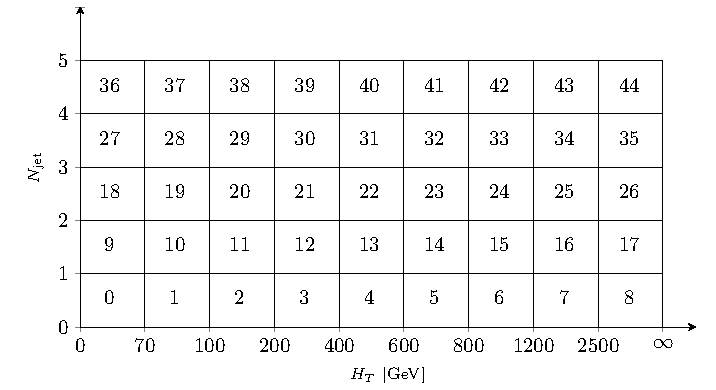
\includegraphics[width=0.48\textwidth]{plots/regions_WJets_vs_Njet_and_HT.pdf}
\caption{
  Definition of the PS regions $i$ in the plane of $N_{\jet}$ versus $\HT$,
  %for the case that $\PW \to \Plepton\Pnu$ samples generated at LO accuracy in pQCD are stitched based on the observables $N_{\jet}$ and $\HT$.
  for the case of $\PW \to \Plepton\Pnu$ samples that are stitched based on the observables $N_{\jet}$ and $\HT$.
}
\label{fig:regions_WJets_vs_Njet_and_HT}
\end{figure}

\begin{figure*}
\setlength{\unitlength}{1mm}
\begin{center}
\begin{picture}(180,182)(0,0)
\put(8.5, 100.0){\mbox{\includegraphics*[height=82mm]{plots/WJets_lead_stack_wRatio_log.pdf}}}
\put(96.5, 100.0){\mbox{\includegraphics*[height=82mm]{plots/WJets_sublead_stack_wRatio_log.pdf}}}
\put(8.5, 4.0){\mbox{\includegraphics*[height=82mm]{plots/WJets_njet_stack_wRatio_log.pdf}}}
\put(96.5, 4.0){\mbox{\includegraphics*[height=82mm]{plots/WJets_ht_stack_wRatio_log.pdf}}}
\put(45.0, 96.0){\small (a)}
\put(133.0, 96.0){\small (b)}
\put(45.0, 0.0){\small (c)}
\put(133.0, 0.0){\small (d)}
\end{picture}
\end{center}
\caption{
  Distributions in $\pT$ of the (a) leading and (b) subleading jet,
  in (c) the multiplicity of jets and in (d) the observable $\HT$,
  %for the case that $\PW \to \Plepton\Pnu$ samples generated at LO accuracy in pQCD are stitched based on the observables $N_{\jet}$ and $\HT$.
  for the case of $\PW \to \Plepton\Pnu$ samples that are stitched based on the observables $N_{\jet}$ and $\HT$.
  The event yields are computed for an integrated luminosity of $140\fbinv$.
}
\label{fig:controlPlots_WJets_vs_Njet_and_HT}
\end{figure*}


\subsection{Estimation of trigger rate}
\label{sec:examples_trigger_rate}

The application of the stitching procedure to the case of estimating trigger rates at the HL-LHC demonstrates the flexibility of our formalism.
As mentioned in Section~\ref{sec:examples}, the probability $P^{I} = P^{i_{1},\dots,i_{N_{\pileup}+1}}$ follows a multinomial distribution in this example.
The symbol $N_{\pileup}$ denotes the number of pileup (PU) interactions 
that occur in the same crossing of the proton beams as the hard-scatter (HS) interaction. 
The distinction between the HS interaction and the PU is artificial and is solely made for the purpose of MC production:
The HS interaction as well as the PU are of the same kind of inelastic $\Pp\Pp$ scatterings,
predominantly arising from the exchange of gluons between the colliding protons,
and solely differ by the transverse momentum $\pThat$ that is exchanged in the scattering.

The ``inclusive'' sample in this example are events containing $N_{\pileup} + 1$ minimum bias interactions,
where for each event the number of PU interactions, $N_{\pileup}$, is sampled at random from the Poisson probability distribution:
\begin{equation}
\Poisson(N_{\pileup} \vert \Nbar) = \frac{\Nbar^{N_{\pileup}} \times e^{-\Nbar}}{N_{\pileup}!}
\label{eq:Poisson}
\end{equation}

with a mean $\Nbar = 200$.
The exclusive samples contain one HS interaction of transverse momentum within a specified range in $\pThat$ and $N_{\pileup}$ additional minimum bias interactions to simulate the PU.
The number $N_{\pileup}$ of PU interactions is again sampled at random from a Poisson distribution with a mean of $\Nbar = 200$.

We enumerate the ranges in $\pThat$ by the index $i$ and denote the number of $\pThat$ ranges used to produce the exclusive samples by the symbol $k$.
We further use the symbol $n_{i}$ to refer to the number of inelastic $\Pp\Pp$ scatterings,
occurring either in the HS interaction or in any of the $N_{\pileup}$ PU interactions,
which fall into the $i$-th interval in $\pThat$.

The probability $P^{I}$ for an event in the inclusive sample that contains $N_{\pileup}$ pileup interactions
to feature $n_{1}$ inelastic $\Pp\Pp$ scatterings that fall into the first interval in $\pThat$, $n_{2}$ into the second,$\dots$, and $n_{k}$ into the $k$-th 
is given by:
\begin{equation}
P^{I} = \frac{(N_{\pileup} + 1)!}{n_{1}! \times \dots \times n_{k}!} \times p_{1}^{n_{1}} \times \dots \times p_{k}^{n_{k}} \, ,
\label{eq:P_inclusive}
\end{equation}
where the symbols $p_{i}$ correspond to the probability for a single inelastic $\Pp\Pp$ scattering interaction to feature a transverse momentum exchange that falls into the $i$-th interval in $\pThat$.
The $n_{i}$ satisfy the condition $\sum_{i=1}^{k} \, n_{i} = N_{\pileup} + 1$.

The corresponding probability $P_{j}^{I}$ for an event in the $j$-th exclusive sample that contains $N_{\pileup}$ pileup interactions is given by:
\begin{equation}
P_{j}^{I} = \begin{cases}\!
\begin{aligned}[b]
 \frac{N_{\pileup}!}{n_{1}! \times \dots \times (n_{j} - 1)! \times \dots \times n_{k}!} \times \\ 
  \quad p_{1}^{n_{1}} \times \dots \times p_{j}^{(n_{j} - 1)} \times \dots \times p_{k}^{n_{k}} \, ,
\end{aligned} & \text{if $n_{j} \geq 1$} \\
0 \, , & \text{otherwise} \, .
\end{cases}
\label{eq:P_exclusive}
\end{equation}
The $n_{i}$ again satisfy the condition $N_{\pileup} + 1 = \sum_{i=1}^{k} \, n_{i}$.
The fact that for all events in the $j$-th exclusive sample the transverse momentum $\pThat$ exchanged in the HS interaction falls into the $j$-th interval in $\pThat$
implies that $N_{\pileup} + 1$ needs to be replaced by $N_{\pileup}$ and $n_{j}$ by $n_{j} - 1$ in Eq.~(\ref{eq:P_exclusive}) compared to Eq.~(\ref{eq:P_inclusive}),
as one of the inelastic $\Pp\Pp$ scatterings that fall into the $j$-th interval in $\pThat$ is ``fixed'' and thus not subject to the random fluctuations, which are modeled by the multinomial distribution.
The ratio of Eq.~(\ref{eq:P_exclusive}) to Eq.~(\ref{eq:P_inclusive}) is given by the expression:
\begin{equation}
\frac{P_{j}^{I}}{P^{I}} = \frac{n_{j}}{(N_{\pileup} + 1) \times p_{j}} \, .
\label{eq:P_ratio}
\end{equation}
The validity of Eq.~(\ref{eq:P_ratio}) includes the case $n_{j} = 0$.

The expression for the stitching weight $w^{I}$ is given by an expression similar to Eq.~(\ref{eq:weight_incl}),
the main difference being that the index $i$ is replaced by the vector $I$,
the probabilities $P^{i}$ and $P_{j}^{i}$ are replaced by the probabilities $P^{I}$ and $P_{j}^{I}$
and the product of luminosity times cross section, $L \times \sigma_{\incl}$, is replaced by the frequency $F$ of $\Pp\Pp$ collisions 
for the purpose of estimating trigger rates at the HL-LHC:
\begin{equation}
w^{I} = \frac{F}{N_{\incl}} \times \frac{N_{\incl} \times P^{I}}{N_{\incl} \times P^{I} + \sum_{j} \, N_{j} \times P_{j}^{I}} \, .
\label{eq:weight_tmp}
\end{equation}
The probabilities $P^{I}$ and $P_{j}^{I}$ are given by Eqs.(~\ref{eq:P_inclusive}) and~(\ref{eq:P_exclusive}).
Dividing both numerator and denominator on the right-hand side of Eq.~(\ref{eq:weight_tmp}) by $P^{I}$ and replacing the ratio $P_{j}^{I}/P^{I}$ by Eq.~(\ref{eq:P_ratio}) yields:
\begin{equation}
w^{I} = \frac{F}{N_{\incl} + \sum_{j} \, N_{j} \times \frac{n_{j}}{(N_{\pileup} + 1) \times p_{j}}} \, .
\label{eq:weight_trigger_rate}
\end{equation}
At the HL-LHC, the $\Pp\Pp$ collision frequency $F$ amounts to $28$~MHz~\footnote{
  The beams cross every $25$~ns, but $\Pp\Pp$ collisions occur only in $\approx 70\%$ of those beam crossings~\cite{TDR_Phase2_LHC}.}.
Eq.~(\ref{eq:weight_trigger_rate}) represents the equivalent of Eq.~(\ref{eq:weight_incl}),
tailored to the case of estimating trigger rates instead of estimating event yields of background processes.

The ranges in $\pThat$ used to produce the exclusive samples and the number of events contained in each sample
are given in Table~\ref{tab:samples_trigger_rate}.
The association of the index $i$ to the different ranges in $\pThat$ and the 
corresponding values of the probabilities $p_{i}$ are given in Table~\ref{tab:p_trigger_rate}.
The probabilities $p_{i}$ are computed by taking the ratio of cross sections computed by the program \PYTHIA
for the case of single inelastic $\Pp\Pp$ scattering interactions with a transverse momentum exchange that is within the $i$-th interval in $\pThat$
and for the case that no condition is imposed on $\pThat$.

\begin{table}
\caption{
  Number of events in the inclusive and exclusive samples used to estimate trigger rates at the HL-LHC.
}
\label{tab:samples_trigger_rate}
\begin{center}
\begin{tabular}{l|c}
\hline
Sample                    & Number of events \\
\hline
Inclusive                 & $8 \times 10^{5}$ \\
\hline
$ 30 < \pThat <  50$~\GeV & $4 \times 10^{5}$ \\
$ 50 < \pThat <  80$~\GeV & $2 \times 10^{5}$ \\
$ 80 < \pThat < 120$~\GeV & $1 \times 10^{5}$ \\
$120 < \pThat < 170$~\GeV & $5 \times 10^{4}$ \\
$170 < \pThat < 300$~\GeV & $5 \times 10^{4}$ \\
$300 < \pThat < 470$~\GeV & $5 \times 10^{4}$ \\
$470 < \pThat < 600$~\GeV & $5 \times 10^{4}$ \\
$\pThat > 600$~\GeV       & $5 \times 10^{4}$ \\
\hline
\end{tabular}
\end{center}
\end{table}

\begin{table*}
\caption{
  Probabilities $p_{i}$ for a single inelastic $\Pp\Pp$ scattering interaction to feature a transverse momentum exchange 
  between the protons that is within the $i$-th interval in $\pThat$.
}
\label{tab:p_trigger_rate}
\begin{center}
%\small
\begin{minipage}{16cm}
\begin{tabular}{l|cccccc}
\hline
Range in $\pThat$ [\GeV] & $< 30$ & $30$-$50$ & $50$-$80$ & $80$-$120$ & $120$-$170$ & $170$-$300$ \\
Index $i$           & $0$ & $1$ & $2$ & $3$ & $4$ & $5$ \\
\hline
\hline
Probability $p_{i}$ & $0.998$ & $1.51 \times 10^{-3}$ & $2.25 \times 10^{-4}$ & $3.38 \times 10^{-5}$ & $6.00 \times 10^{-6}$ & $1.55 \times 10^{-6}$ \\
\hline
\end{tabular}

\vspace{2mm}

\begin{tabular}{l|ccc}
\hline
Range in $\pThat$ [\GeV] & $300$-$470$ & $470$-$600$ & $> 600$ \\
Index $i$           & $6$ & $7$ & $8$ \\
\hline
\hline
Probability $p_{i}$ & $1.05 \times 10^{-7}$ & $8.73 \times 10^{-9}$ & $3.12 \times 10^{-9}$ \\
\hline
\end{tabular}
\end{minipage}
\end{center}
\end{table*}

We cannot give numerical values of the weights $w^{I}$ for this example,
as $I$ is a high-dimensional vector, and also because the weights $w^{I}$ vary depending on $N_{\pileup}$.
Instead, we show in Fig.~\ref{fig:weight_trigger_rate} the spectrum of the weights $w^{I}$
that we obtain when inserting the numbers given in Tables~\ref{tab:samples_trigger_rate} and~\ref{tab:p_trigger_rate} into Eq.~(\ref{eq:weight_trigger_rate}).
For comparison, we also show the corresponding weight, given by $w_{\incl} = F/N_{\incl}$,
for the case that only the inclusive sample is used to estimate the trigger rate.
The weight $w_{\incl}$ amounts to $35$~Hz in this example.
As can be seen in Fig.~\ref{fig:weight_trigger_rate}, the addition of samples produced in ranges in $\pThat$ to the inclusive sample reduces the weights.
The different maxima in the distribution of stitching weights $w^{I}$ correspond to events 
in which the transverse momentum exchanged between the scattered protons falls into different ranges in $\pThat$.
The spectrum of weights shown in Fig.~\ref{fig:weight_trigger_rate} is plotted before any trigger selection is applied.
The stitching weights $w^{I}$ are on average smaller for events that pass than for events that fail the trigger selection,
as the probability for an event to pass the trigger increases with $\pThat$.
In contrast, the weights $w_{\incl}$ are the same before and after the trigger selection is applied.
The reduction in weights thus becomes more pronounced after the trigger selection is applied.

\begin{figure}
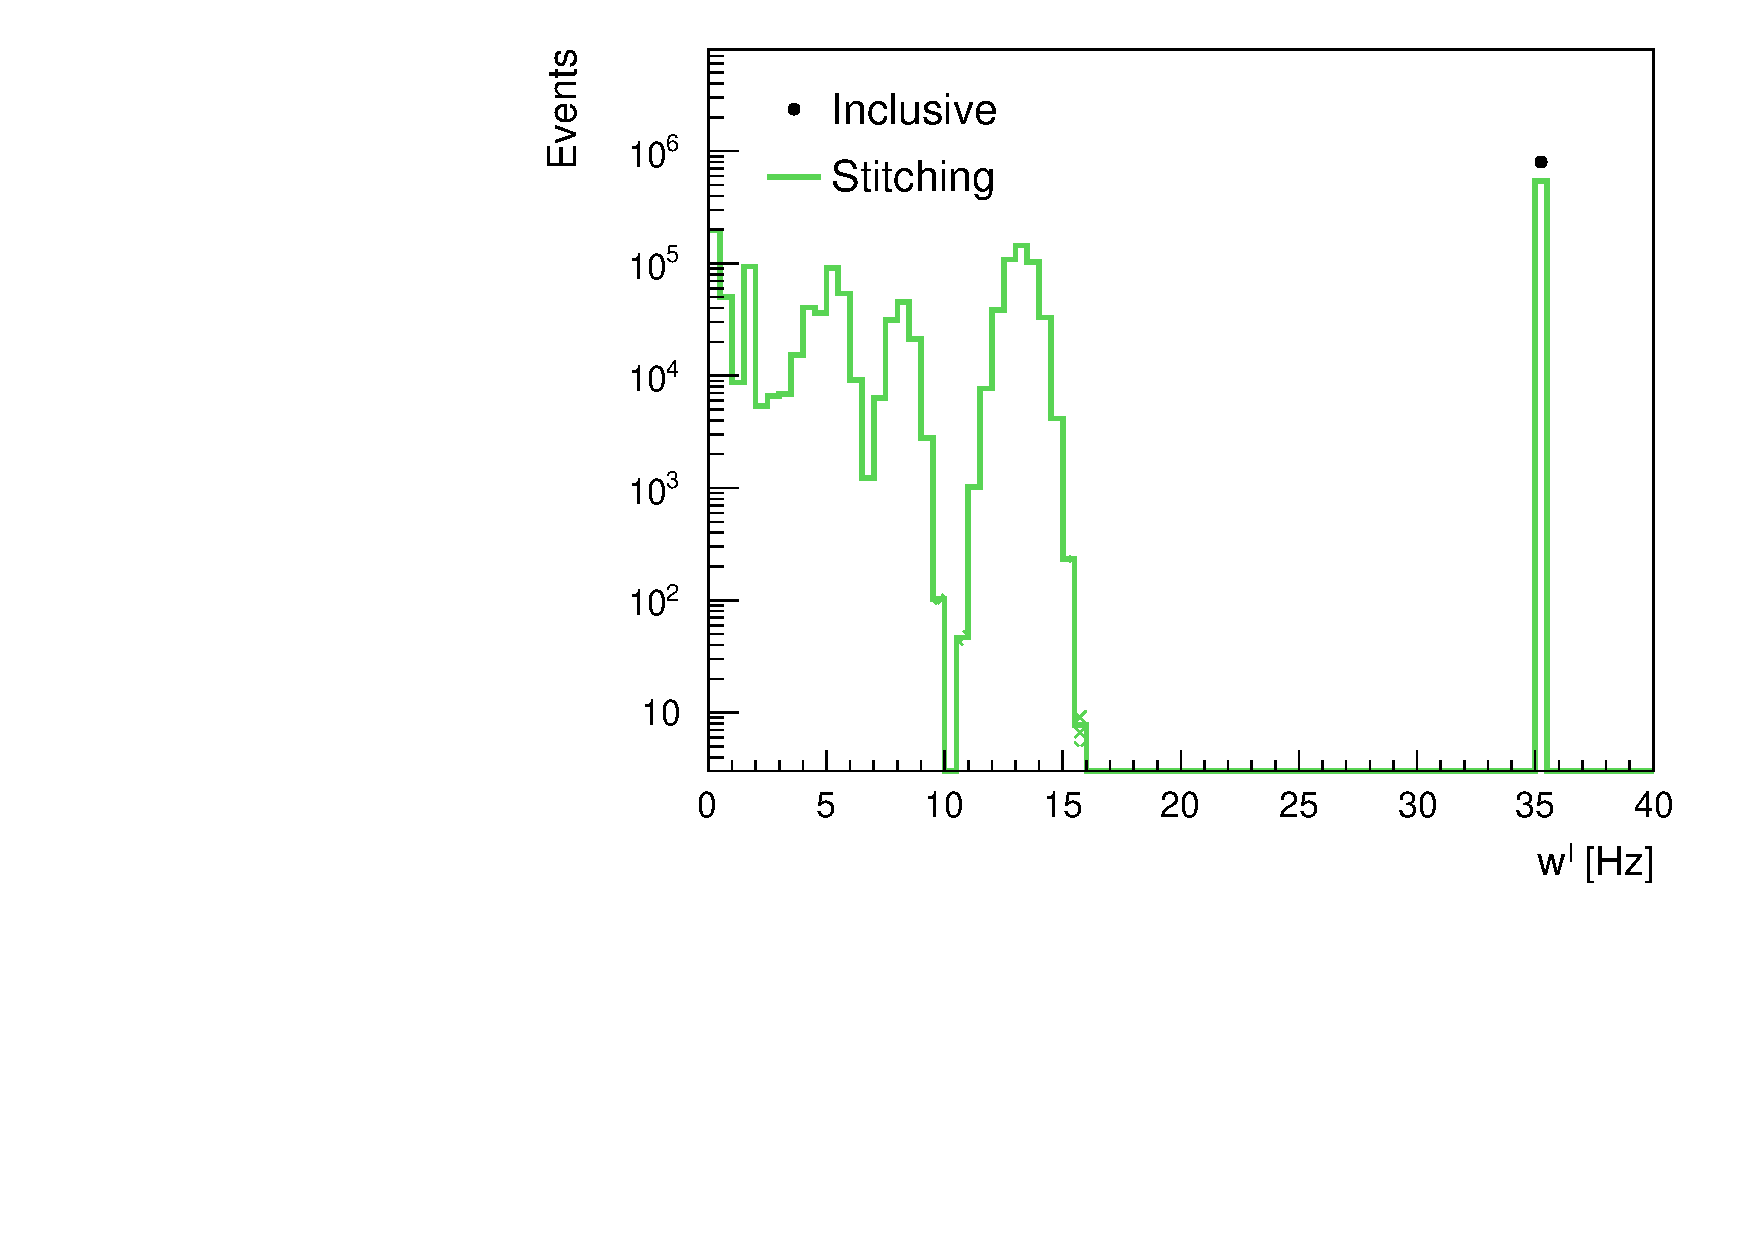
\includegraphics[width=0.48\textwidth]{plots/makeEvtWeightPlotsForPaper_evtWeight_log.pdf}
\caption{
  Weights $w^{I}$, computed according to Eq.~(\ref{eq:weight_trigger_rate}), 
  for the inclusive sample and for the samples produced in ranges of $\pThat$.
}
\label{fig:weight_trigger_rate}
\end{figure}

The rates expected for a single jet trigger and for a dijet trigger at the HL-LHC are shown in Fig.~\ref{fig:trigger_rate}.
The rates are computed as function of the $\pT$ threshold that is applied to the jets. 
In case of the dijet trigger, the same $\pT$ threshold is applied to both jets.
The jets are required to be within the geometric acceptance $\vert\eta\vert < 5.0$.
The rate estimates obtained for the inclusive sample and for the sum of inclusive plus exclusive samples, 
with the stitching weights computed according to Eq.~(\ref{eq:weight_trigger_rate}),
agree within statistical uncertainties, demonstrating that the estimate of the trigger rate obtained from the stitching procedure is unbiased.
The statistical uncertainties on the rate estimates obtained from the inclusive sample are represented by error bars,
while those obtained from the sum of inclusive plus exclusive samples are represented by the shaded area.

\begin{figure*}
\setlength{\unitlength}{1mm}
\begin{center}
\begin{picture}(180,90)(0,0)
\put(8.5, 4.0){\mbox{\includegraphics*[height=86mm]
  {plots/makeRatePlotsForPaper_SingleJet_absEtaLt5p00_log.pdf}}}
\put(96.5, 4.0){\mbox{\includegraphics*[height=86mm]
  {plots/makeRatePlotsForPaper_DoubleJet_absEtaLt5p00_log.pdf}}}
\put(47.0, 0.0){\small (a)}
\put(135.0, 0.0){\small (b)}
\end{picture}
\end{center}
\caption{
  Rate expected for (a) a single jet trigger and (b) a dijet trigger at the HL-LHC, as function of the $\pT$ threshold that is applied to the jets.
}
\label{fig:trigger_rate}
\end{figure*}

The statistical uncertainties obtained with the stitching procedure are smaller than the ones obtained in case only the inclusive sample is used.
The reduction in the statistical uncertainties is more pronounced for the dijet trigger than for the single jet trigger.
The single jet trigger rate decreases only modestly for jet $\pT$ thresholds greater than $400$~\GeV.
This ``flattening'' of the trigger rate is due to events with low $\pThat$ that contain a single jet of high $\pT$.
The stitching weights $w^{I}$ for these low $\pThat$ events are not much smaller than the weights for the inclusive sample,
which explains why the statistical uncertainties on the single jet trigger rate are reduced only modestly by the stitching procedure.
Thr requirement of a second high $\pT$ jet removes most of these $\pThat$ events.
Consequently, very few low $\pThat$ events pass high jet $\pT$ thresholds in case of the dijet trigger,
with the effect that the dijet trigger rate decreases more rapidly as function of the jet $\pT$ threshold
and the stitching procedure becomes more effective in reducing the statistical uncertainties on the trigger rate.


\section{Summary}
\label{sec:summary}

The production of MC samples of adequate size is often a challenge in modern HEP experiments,
due to the computing resources required to produce and store such samples.
This is particularly true for experiments at the CERN LHC,
firstly because of the large $\Pp\Pp$ scattering cross section and secondly because of the large luminosity delivered by the LHC.

In this paper we have presented a procedure that allows to reduce the statistical uncertainties 
by combining MC samples which overlap in PS.
Our formalism is general enough to be applied in various use-cases.
Different examples for applying the formalism to $\Pp\Pp$ collisions at the LHC are given in this paper.

Of particular interest is the case of modelling background contributions to searches for new physics,
where potential signals are typically expected to be small and often similar in size to the statistical uncertainties on the background contributions.
The statistical uncertainties on these background contributions can often be significantly reduced 
by dividing the PS into multiple regions, producing separate MC samples for each region,
and accounting for the overlap of different samples in PS by applying the weights computed as detailed in this paper to the simulated events.
We refer to this procedure as ``stitching''.

The flexibility of our formalism is demonstrated by applying the stitching procedure to the case of estimating trigger rates at the HL-LHC,
where up to $200$ simultaneous $\Pp\Pp$ collisions are expected per crossing of the proton beams.


%\appendix
%\section{Supplementary material}

\begin{sidewaystable*}
\caption{
  Probabilities $P^{i}$ and $P_{j}^{i}$ for the events in the inclusive and exclusive $\PW \to \Plepton\Pnu$ samples 
  %simulated at LO accuracy in pQCD 
  to populate the different PS regions $i$.
  The definition of the PS regions $i$ in the plane of $N_{\jet}$ versus $\HT$ is shown in Fig.~\ref{fig:regions_WJets_vs_Njet_and_HT}.
  A hyphen ($-$) indicates PS regions $i$ that are not populated by a given sample $j$. The presence of a hyphen is equivalent to the probability $P_{j}^{i}$ being zero.
}
\label{tab:probabilities_WJets_vs_Njet_and_HT}
\centering              
\resizebox{\textwidth}{!}{
\begin{tabular}{lccccccccccccccc}
\hline
Sample                   &  $P^{0}$ &  $P^{1}$ &  $P^{2}$ &  $P^{3}$ &  $P^{4}$ &  $P^{5}$ &  $P^{6}$ &  $P^{7}$ &  $P^{8}$ &  $P^{9}$ &  $P^{10}$         &  $P^{11}$            &  $P^{12}$            & $P^{13}$ & $P^{14}$ \\
\hline
\hline
Inclusive                &  $0.758$ &  $-$     &  $-$     &  $-$     &  $-$     &  $-$     &  $-$     &  $-$     &  $-$     &  $0.156$ &  $6\times10^{-3}$ &  $2.51\times10^{-3}$ &  $1.48\times10^{-4}$ &  $4.02\times10^{-6}$ &  $0$ \\
\hline
$N_{\jet} = 1$           &  $-$ &  $-$ &  $-$ &  $-$ &  $-$ &  $-$ &  $-$ &  $-$ &  $-$ &  $0.948$ &  $3.64\times10^{-2}$ &  $1.52\times10^{-2}$ &  $9.00\times10^{-4}$ &  $2.44\times10^{-5}$ &  $1.87\times10^{-6}$ \\
$N_{\jet} = 2$           &  $-$ &  $-$ &  $-$ &  $-$ &  $-$ &  $-$ &  $-$ &  $-$ &  $-$ &  $-$ &  $-$ &  $-$ &  $-$ &  $-$ &  $-$ \\
$N_{\jet} = 3$           &  $-$ &  $-$ &  $-$ &  $-$ &  $-$ &  $-$ &  $-$ &  $-$ &  $-$ &  $-$ &  $-$ &  $-$ &  $-$ &  $-$ &  $-$ \\
$N_{\jet} = 4$           &  $-$ &  $-$ &  $-$ &  $-$ &  $-$ &  $-$ &  $-$ &  $-$ &  $-$ &  $-$ &  $-$ &  $-$ &  $-$ &  $-$ &  $-$ \\
\hline
$  70 < \HT <  100$~\GeV &  $-$ &  $-$ &  $-$ &  $-$ &  $-$ &  $-$ &  $-$ &  $-$ &  $-$ &  $-$ &  $0.259$ &  $-$ &  $-$ &  $-$ &  $-$ \\
$ 100 < \HT <  200$~\GeV &  $-$ &  $-$ &  $-$ &  $-$ &  $-$ &  $-$ &  $-$ &  $-$ &  $-$ &  $-$ &  $-$ &  $0.109$ &  $-$ &  $-$ &  $-$ \\
$ 200 < \HT <  400$~\GeV &  $-$ &  $-$ &  $-$ &  $-$ &  $-$ &  $-$ &  $-$ &  $-$ &  $-$ &  $-$ &  $-$ &  $-$ &  $2.40\times10^{-2}$ &  $-$ &  $-$ \\
$ 400 < \HT <  600$~\GeV &  $-$ &  $-$ &  $-$ &  $-$ &  $-$ &  $-$ &  $-$ &  $-$ &  $-$ &  $-$ &  $-$ &  $-$ &  $-$ &  $4.82\times10^{-3}$ &  $-$ \\
$ 600 < \HT <  800$~\GeV &  $-$ &  $-$ &  $-$ &  $-$ &  $-$ &  $-$ &  $-$ &  $-$ &  $-$ &  $-$ &  $-$ &  $-$ &  $-$ &  $-$ &  $1.50\times10^{-3}$ \\
$ 800 < \HT < 1200$~\GeV &  $-$ &  $-$ &  $-$ &  $-$ &  $-$ &  $-$ &  $-$ &  $-$ &  $-$ &  $-$ &  $-$ &  $-$ &  $-$ &  $-$ &  $-$ \\
$1200 < \HT < 2500$~\GeV &  $-$ &  $-$ &  $-$ &  $-$ &  $-$ &  $-$ &  $-$ &  $-$ &  $-$ &  $-$ &  $-$ &  $-$ &  $-$ &  $-$ &  $-$ \\
$       \HT > 2500$~\GeV &  $-$ &  $-$ &  $-$ &  $-$ &  $-$ &  $-$ &  $-$ &  $-$ &  $-$ &  $-$ &  $-$ &  $-$ &  $-$ &  $-$ &  $-$ \\
\hline
\hline
Sample                   & $P^{15}$ & $P^{16}$ & $P^{17}$ & $P^{18}$ & $P^{19}$ & $P^{20}$ & $P^{21}$ & $P^{22}$ & $P^{23}$ & $P^{24}$ & $P^{25}$ & $P^{26}$ & $P^{27}$ & $P^{28}$ & $P^{29}$ \\
\hline
\hline
Inclusive                & $8.89\times10^{-8}$ &  $0$ &  $0$ &  $2.84\times10^{-2}$ &  $1.29\times10^{-2}$ &  $9.67\times10^{-3}$ &  $1.23\times10^{-3}$ &  $7.58\times10^{-5}$ &  $1.18\times10^{-5}$ &  $3.36\times10^{-6}$ &  $5.21\times10^{-7}$ &  $0$ &  $1.36\times10^{-3}$ &  $4.03\times10^{-3}$ &  $7.6\times10^{-3}$ \\
\hline
$N_{\jet} = 1$           &  $5.40\times10^{-7}$ &  $0$ &  $0$ &  $-$ &  $-$ &  $-$ &  $-$ &  $-$ &  $-$ &  $-$ &  $-$ &  $-$ &  $-$ &  $-$ &  $-$ \\
$N_{\jet} = 2$           &  $-$ &  $-$ &  $-$ &  $0.543$ &  $0.247$ &  $0.185$ &  $2.36\times10^{-2}$ &  $1.45\times10^{-3}$ &  $2.25\times10^{-4}$ &  $6.43\times10^{-5}$ &  $10^{-5}$ &  $0$ &  $-$ &  $-$ &  $-$ \\
$N_{\jet} = 3$           &  $-$ &  $-$ &  $-$ &  $-$ &  $-$ &  $-$ &  $-$ &  $-$ &  $-$ &  $-$ &  $-$ &  $-$ &  $8.91\times10^{-2}$ &  $0.265$ &  $0.499$ \\
$N_{\jet} = 4$           &  $-$ &  $-$ &  $-$ &  $-$ &  $-$ &  $-$ &  $-$ &  $-$ &  $-$ &  $-$ &  $-$ &  $-$ &  $-$ &  $-$ &  $-$ \\
\hline
$  70 < \HT <  100$~\GeV &  $-$ &  $-$ &  $-$ &  $-$ &  $0.557$ &  $-$ &  $-$ &  $-$ &  $-$ &  $-$ &  $-$ &  $-$ &  $-$ &  $0.174$ &  $-$ \\
$ 100 < \HT <  200$~\GeV &  $-$ &  $-$ &  $-$ &  $-$ &  $-$ &  $0.421$ &  $-$ &  $-$ &  $-$ &  $-$ &  $-$ &  $-$ &  $-$ &  $-$ &  $0.331$ \\
$ 200 < \HT <  400$~\GeV &  $-$ &  $-$ &  $-$ &  $-$ &  $-$ &  $-$ &  $0.200$ &  $-$ &  $-$ &  $-$ &  $-$ &  $-$ &  $-$ &  $-$ &  $-$ \\
$ 400 < \HT <  600$~\GeV &  $-$ &  $-$ &  $-$ &  $-$ &  $-$ &  $-$ &  $-$ &  $9.09\times10^{-2}$ &  $-$ &  $-$ &  $-$ &  $-$ &  $-$ &  $-$ &  $-$ \\
$ 600 < \HT <  800$~\GeV &  $-$ &  $-$ &  $-$ &  $-$ &  $-$ &  $-$ &  $-$ &  $-$ &  $5.72\times10^{-2}$ &  $-$ &  $-$ &  $-$ &  $-$ &  $-$ &  $-$ \\
$ 800 < \HT < 1200$~\GeV &  $1.02\times10^{-4}$ &  $-$ &  $-$ &  $-$ &  $-$ &  $-$ &  $-$ &  $-$ &  $-$ &  $3.87\times10^{-2}$ &  $-$ &  $-$ &  $-$ &  $-$ &  $-$ \\
$1200 < \HT < 2500$~\GeV &  $-$ &  $9.02\times10^{-4}$ &  $-$ &  $-$ &  $-$ &  $-$ &  $-$ &  $-$ &  $-$ &  $-$ &  $2.12\times10^{-2}$ &  $-$ &  $-$ &  $-$ &  $-$ \\
$       \HT > 2500$~\GeV &  $-$ &  $-$ &  $0$ &  $-$ &  $-$ &  $-$ &  $-$ &  $-$ &  $-$ &  $-$ &  $-$ &  $0$ &  $-$ &  $-$ &  $-$ \\
\hline
\hline
Sample                   & $P^{30}$ & $P^{31}$ & $P^{32}$ & $P^{33}$ & $P^{34}$ & $P^{35}$ & $P^{36}$ & $P^{37}$ & $P^{38}$ & $P^{39}$ & $P^{40}$ & $P^{41}$ & $P^{42}$ & $P^{43}$ & $P^{44}$ \\
\hline
\hline
Inclusive                &  $1.94\times10^{-3}$ &  $1.70\times10^{-4}$ &  $2.98\times10^{-5}$ &  $9.17\times10^{-6}$ &  $1.46\times10^{-6}$ &  $0$ &  $1.39\times10^{-5}$ &  $2.96\times10^{-4}$ &  $3.24\times10^{-3}$ &  $2.83\times10^{-3}$ &  $5.76\times10^{-4}$ &  $1.60\times10^{-4}$ &  $7.20\times10^{-5}$ &  $2.13\times10^{-5}$ &  $0$ \\
\hline
$N_{\jet} = 1$           &  $-$ &  $-$ &  $-$ &  $-$ &  $-$ &  $-$ &  $-$ &  $-$ &  $-$ &  $-$ &  $-$ &  $-$ &  $-$ &  $-$ &  $-$ \\
$N_{\jet} = 2$           &  $-$ &  $-$ &  $-$ &  $-$ &  $-$ &  $-$ &  $-$ &  $-$ &  $-$ &  $-$ &  $-$ &  $-$ &  $-$ &  $-$ &  $-$ \\
$N_{\jet} = 3$           &  $0.127$ &  $1.12\times10^{-2}$ &  $1.95\times10^{-3}$ &  $6.02\times10^{-4}$ &  $9.60\times10^{-5}$ &  $0$ &  $-$ &  $-$ &  $-$ &  $-$ &  $-$ &  $-$ &  $-$ &  $-$ &  $-$ \\
$N_{\jet} = 4$           &  $-$ &  $-$ &  $-$ &  $-$ &  $-$ &  $-$ &  $1.93\times10^{-3}$ &  $4.12\times10^{-2}$ &  $0.451$ &  $0.393$ &  $7.99\times10^{-2}$ &  $2.23\times10^{-2}$ &  $10^{-2}$ &  $2.95\times10^{-3}$ &  $1.18\times10^{-4}$ \\
\hline
$  70 < \HT <  100$~\GeV &  $-$ &  $-$ &  $-$ &  $-$ &  $-$ &  $-$ &  $-$ &  $1.28\times10^{-2}$ &  $-$ &  $-$ &  $-$ &  $-$ &  $-$ &  $-$ &  $-$ \\
$ 100 < \HT <  200$~\GeV &  $-$ &  $-$ &  $-$ &  $-$ &  $-$ &  $-$ &  $-$ &  $-$ &  $0.141$ &  $-$ &  $-$ &  $-$ &  $-$ &  $-$ &  $-$ \\
$ 200 < \HT <  400$~\GeV &  $0.314$ &  $-$ &  $-$ &  $-$ &  $-$ &  $-$ &  $-$ &  $-$ &  $-$ &  $0.459$ &  $-$ &  $-$ &  $-$ &  $-$ &  $-$ \\
$ 400 < \HT <  600$~\GeV &  $-$ &  $0.204$ &  $-$ &  $-$ &  $-$ &  $-$ &  $-$ &  $-$ &  $-$ &  $-$ &  $0.690$ &  $-$ &  $-$ &  $-$ &  $-$ \\
$ 600 < \HT <  800$~\GeV &  $-$ &  $-$ &  $0.145$ &  $-$ &  $-$ &  $-$ &  $-$ &  $-$ &  $-$ &  $-$ &  $-$ &  $0.781$ &  $-$ &  $-$ &  $-$ \\
$ 800 < \HT < 1200$~\GeV &  $-$ &  $-$ &  $-$ &  $0.106$ &  $-$ &  $-$ &  $-$ &  $-$ &  $-$ &  $-$ &  $-$ &  $-$ &  $0.830$ &  $-$ &  $-$ \\
$1200 < \HT < 2500$~\GeV &  $-$ &  $-$ &  $-$ &  $-$ &  $5.95\times10^{-2}$ &  $-$ &  $-$ &  $-$ &  $-$ &  $-$ &  $-$ &  $-$ &  $-$ &  $0.865$ &  $-$ \\
$       \HT > 2500$~\GeV &  $-$ &  $-$ &  $-$ &  $-$ &  $-$ &  $0$ &  $-$ &  $-$ &  $-$ &  $-$ &  $-$ &  $-$ &  $-$ &  $-$ &  $1$ \\
\hline
\end{tabular}
}
\end{sidewaystable*}

\begin{table*}
\caption{
  Weights $w^{i}$ for the case that the inclusive and exclusive $\PW \to \Plepton\Pnu$ samples 
  given in 
  %Tables~\ref{tab:samples_and_probabilities_WJets_vs_Njet} and~\ref{tab:samples_WJets_vs_Njet_and_HT}
  Tables~\ref{tab:samples_WJets_vs_Njet} and~\ref{tab:samples_WJets_vs_Njet_and_HT}
  %, simulated at LO accuracy in pQCD,
  are stitched based on the observables $N_{\jet}$ and $\HT$.
  The weights are computed for an integrated luminosity of $140\fbinv$.
  Events with $N_{\jet} = 0$ all have $\HT < 70$~\GeV and hence the weights for PS regions with $N_{\jet} = 0$ and $\HT \geqslant 70$~\GeV cannot be computed (and are not needed).
  These cases are indicated by a hyphen ($-$).
  %The definition of the PS regions $i$ in the plane of $N_{\jet}$ versus $\HT$ is shown in Fig.~\ref{fig:regions_WJets_vs_Njet_and_HT}.
}
\label{tab:weights_WJets_vs_Njet_and_HT}
\begin{center}
\begin{tabular}{l|c|c|c|c|c}
\hline
                                 & $N_{\jet} = 0$ & $N_{\jet} = 1$      & $N_{\jet} = 2$      & $N_{\jet} = 3$      & $N_{\jet} = 4$       \\ 
\hline
               $\HT < 70$~\GeV   & $2870$         &  $263$              & $256$              & $260$              &  $257$  \\
  $70 \leqslant \HT < 100$~\GeV  & $-$            &  $137$              & $135$              & $136$              &  $135$  \\
 $100 \leqslant \HT < 200$~\GeV  & $-$            &  $137$              & $135$              & $136$              &  $136$  \\
 $200 \leqslant \HT < 400$~\GeV  & $-$            &  $135$              & $134$              & $135$              &  $134$  \\
 $400 \leqslant \HT < 600$~\GeV  & $-$            &  $132$              & $133$              & $134$              &  $134$  \\
 $600 \leqslant \HT < 800$~\GeV  & $-$            &  $140$              & $135$              & $136$              &  $139$  \\
 $800 \leqslant \HT < 1200$~\GeV & $-$            &  $109$              & $119$              & $124$              &  $128$  \\
$1200 \leqslant \HT < 2500$~\GeV & $-$            &  $193$              & $109$              & $102$              &  $123$  \\
       $\HT \geqslant 2500$~\GeV & $-$            &    $0$              &   $0$              &   $0$              &  $203$  \\
\hline
\end{tabular}
\end{center}
\end{table*}


\begin{acknowledgements}
%If you'd like to thank anyone, place your comments here
%and remove the percent signs.
This work was supported by the Estonian Research Council grant PRG445.
\end{acknowledgements}

% BibTeX users please use one of
%\bibliographystyle{spbasic}      % basic style, author-year citations
\bibliographystyle{spmpsci}      % mathematics and physical sciences
%\bibliographystyle{unsrt}
%\bibliographystyle{spphys}       % APS-like style for physics
\bibliography{mcStitching_epjc}   % name your BibTeX data base

% Non-BibTeX users please use
%\begin{thebibliography}{}
%
% and use \bibitem to create references. Consult the Instructions
% for authors for reference list style.
%
%\bibitem{RefJ}
% Format for Journal Reference
%Author, Article title, Journal, Volume, page numbers (year)
% Format for books
%\bibitem{RefB}
%Author, Book title, page numbers. Publisher, place (year)
% etc
%\end{thebibliography}

\end{document}
% end of file template.tex

